Bei einem Spannungsabfall eines Kondensators werden Wertepaare genommen.
Diese sind in der Tabelle \ref{tab:entladekurve} aufgelistet.
In einem halblogarithmischen Diagramm werden die Wertepaare dargestellt.
Durch eine lineare Ausgleichsgerade kann in der Abbildung \ref{fig:entladekurve} die Steigung ermittelt werden.
Über die Gleichung \eqref{eqn:Entladekurve} lässt sich $RC$ bestimmen.
Die entsprechende Ausgleichsrechnung hat die Form:
\begin{equation*}
  \ln{ \left( \frac{U_c}{U_0} \right)}=-\frac{1}{RC}\cdot t+b.
\end{equation*}
Die Parameter ergeben sich zu:
\begin{align*}
  RC &=& \SI{1.57\pm 0.60e-3}{s}\\
  b  &=& \SI{2.78 \pm 3.53323839e-03}{}.\\
\end{align*}
%\documentclass[captions=tableheading]{scrartcl}
%\usepackage{booktabs}
%\usepackage{pdflscape}
%\usepackage{math}



%\begin{document}
%\begin{landscape}


\begin{table}
  \centering
  \caption{Messdaten zur Entladekurve}
  \label{tab:entladekurve}
  \begin{tabular}{c c c c c c}
    \toprule
     $U_c$/V   & $\ln{\left( \frac{U_c}{U_0} \right)}$ &	T/s	 &    $U_c$/V   & $\ln{\left( \frac{U_c}{U_0} \right)}$ &	T/s	 \\
          \midrule
    19,2	&	-0,0408		 & 	0,0045  & 3,6	  &	-1,7148		 & 	0,0069    \\
    17,2	&	-0,1508		 & 	0,0047  & 3,4	  &	-1,7719		 & 	0,0071    \\
    15,2	&	-0,2744		 & 	0,0048  & 3,0	  & -1,8971	   & 	0,0072    \\
    13,6	&	-0,3857		 & 	0,0050  & 2,8	  &	-1,9661		 & 	0,0074    \\
    12,2	&	-0,4943		 & 	0,0052  & 2,4	  &	-2,1203		 & 	0,0076    \\
    11,0 	&	-0,5978		 & 	0,0053  & 2,2	  &	-2,2073		 & 	0,0077    \\
    9,8	  &	-0,7133		 &  0,0055  & 2,0	  & -2,3026		 & 	0,0079    \\
    8,6	  &	-0,8440		 &  0,0056  & 2,0	  & -2,3026		 & 	0,0080    \\
    7,8	  &	-0,9416		 &  0,0058  & 1,8	  &	-2,4079		 & 	0,0082    \\
    7,0	  & -1,0498	   &  0,0059  & 1,8	  &	-2,4079		 & 	0,0084    \\
    6,4	  &	-1,1394		 &  0,0061  & 1,6	  &	-2,5257		 & 	0,0085    \\
    5,6	  &	-1,2730		 &  0,0063  & 1,4	  &	-2,6593		 & 	0,0087    \\
    5,2	  &	-1,3471		 &  0,0064  & 1,0   &	-2,9957		 & 	0,0088    \\
    4,6	  &	-1,4697		 & 	0,0066  & 1,0   &	-2,9957		 & 	0,0090    \\
    4,2	  &	-1,5606		 & 	0,0068  & 1,0   &	-2,9957		 & 	0,0092    \\

    \bottomrule
  \end{tabular}
\end{table}

%\end{landscape}
%\end{document}

\begin{figure}[h!]
  \centering
  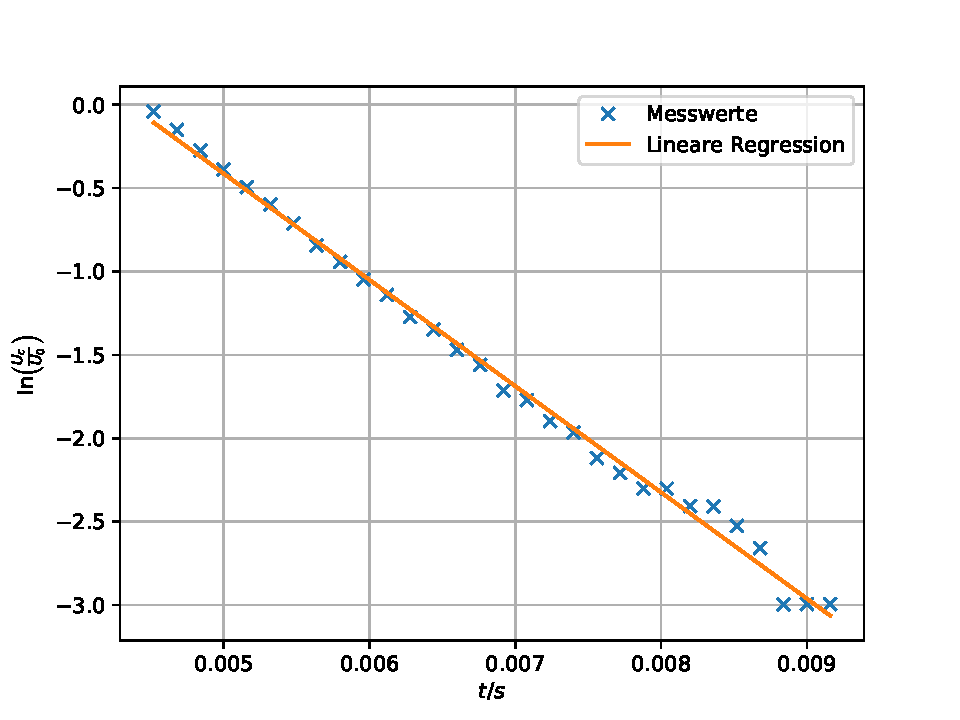
\includegraphics[width=0.8\textwidth]{Zeit.pdf}
  \caption{Lineare Regression zur Bestimmung der Zeitkonstanten mithilfe der Entladekurve}
  \label{fig:entladekurve}
\end{figure}
%\FloatBarrier
%
%
Die nächste Methode zur Bestimmung der Zeitkonstanten erfolgt mit Hilfe der Freqenz und der anliegenden Spannung der Wechselspannungsquelle. Die Werte sind in der Tabelle 2 aufgeführt.
Über die Abbildung \ref{fig:frequenz} und einer Ausgleichsrechnung, mit Hilfe von Gleichung \eqref{eqn:ampkond} lässt sich der Wert für die Zeitkonstante bestimmen.\\
Die Ausgleichsrechnung hat die Form:
\begin{equation*}
    U_{c}=exp(-af+b).
\end{equation*}
Als Parameter ergeben sich:
\begin{align*}
  a &=& \SI{0.00309 \pm 0.00014}{}\\
  b &=& \SI{2.29120 \pm 0.01529}{}.\\
\end{align*}
Damit ergibt sich
\begin{equation*}
  RC = \SI{3.09\pm0.14e-3}{s}
\end{equation*}
%\documentclass[captions=tableheading]{scrartcl}
%\usepackage{booktabs}
%\usepackage{pdflscape}




%\begin{document}
%\begin{landscape}


\begin{table}
  \centering
  \caption{Messdaten zur Frequenz}
  \label{tab:frequenz}
  \begin{tabular}{c c c c}
    \toprule
     $U_c$/V  &		$f/Hz$		&  $U_c$/V  &		$f/Hz$	 \\
          \midrule
    9,2    &   10   &  1,72	   &  600    \\
    9,4    &   20   &  1,48	   &  700    \\
    9,2    &   30   &  1,32	   &  800    \\
    9,0    &   40   &  1,18	   &  900    \\
    8,6    &   50   &  1,06	   &  1000   \\
    8,2    &   60   &  0,536   & 	2000   \\
    8,2    &   70   &  0,360   & 	3000   \\
    8,0    &   80   &  0,264   & 	4000   \\
    7,44	 &   90   &  0,212   & 	5000   \\
    7,12	 &  100   &  0,176   & 	6000   \\
    4,64	 &  200   &  0,152   & 	7000   \\
    3,32	 &  300   &  0,134   & 	8000   \\
    2,60	 &  400   &  0,120   & 	9000   \\
    2,12	 &  500   &  0,106   & 	10000  \\
    1,72	 &  600   &  0,0544  & 	20000  \\
    1,48	 &  700   &  0,0368  & 	30000  \\


    \bottomrule
  \end{tabular}
\end{table}

%\end{landscape}
%\end{document}

\begin{figure}
  \centering
  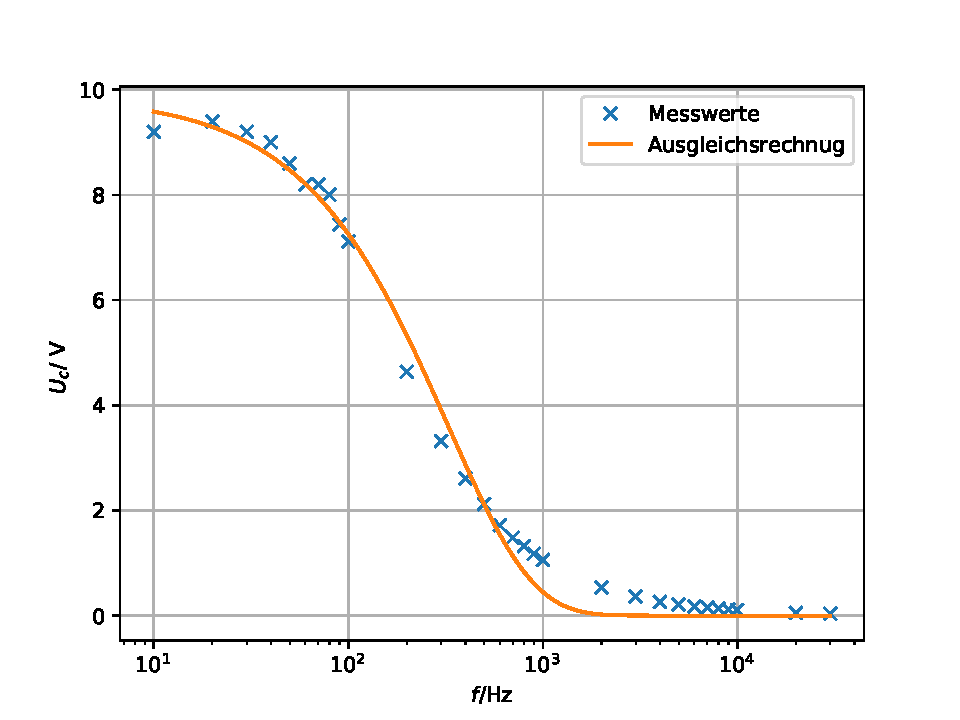
\includegraphics[width=0.8\textwidth]{Freq.pdf}
  \caption{Ausgleichsrechnung zur Bestimmung der Zeitkonstanten mithilfe der Messung der Frequenz}
  \label{fig:frequenz}
\end{figure}
%\FloatBarrier
%
%
In einer dritten Methode wird die Zeitkonstante mit Hilfe der Phasenverschiebung zwischen Generatorspannung und Kondensatorspannung ermittelt. Die bestimmung der Phasenverschiebung
$\phi$ erfolgt über die Formel \eqref{eqn:phasenverschiebung}.
%\begin{equation*}
%  \frac{a}{b}\cdot2\pi=\phi.
%\end{equation*}
Die Werte sind in der Tabelle \ref{tab:phasenverschiebung} aufgeführt.
Die Ausgleichsrechnung hat die Form
\begin{equation*}
   \phi= a\arctan{(bx)}.
\end{equation*}
Als Parameter ergeben sich:
\begin{align*}
  a &=& \SI{0.99991152\pm0.015781563484}{}\\
  b &=& \SI{0.00816372\pm0.000586744095}{}.\\
\end{align*}
Für RC ergibt sich ein Wert von
\begin{equation*}
   RC =  \SI{8.16372 \pm 0.58674e-3}{s}.
\end{equation*}
%\documentclass[captions=tableheading]{scrartcl}
%\usepackage{booktabs}
%\usepackage{pdflscape}
%\usepackage{math}



%\begin{document}
%\begin{landscape}


\begin{table}
  \centering
  \caption{Messdaten zur Phasenverschiebung}
  \label{tab:phasenverschiebung}
  \begin{tabular}{c c c c}
    \toprule
     $\phi$/rad  &	$f$/Hz		&    $\phi$/rad  &	$f$/Hz		  \\
          \midrule
          0,1309   &     10     &       1,3792   &     600      \\
          0,2094   &     20     &       1,4362   &     700      \\
          0,3142   &     30     &       1,4420   &     800      \\
          0,3142   &     40     &       1,5126   &     900      \\
          0,2618   &     50     &       1,5387   &     1000     \\
          0,4712   &     60     &       1,7511   &     2000     \\
          0,5544   &     70     &       1,5708   &     3000     \\
          0,6283   &     80     &       1,4661   &     4000     \\
          0,6981   &     90     &       1,4105   &     5000     \\
          0,6545   &     100    &       1,4137   &     6000     \\
          0,9425   &     200    &       1,5259   &     7000     \\
          1,0996   &     300    &       1,6480   &     8000     \\
          1,2360   &     400    &       1,5126   &     9000     \\
          1,2823   &     500    &       1,5387   &     10000    \\
    \bottomrule
  \end{tabular}
\end{table}

%\end{landscape}
%\end{document}

\begin{figure}
  \centering
  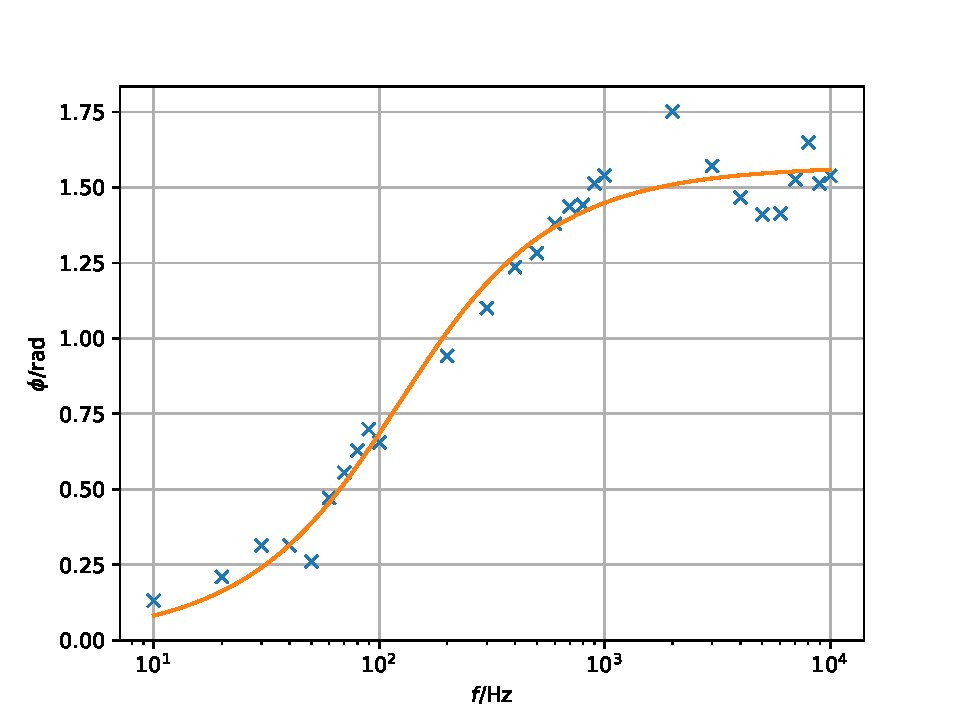
\includegraphics[width=0.8\textwidth]{Polar.pdf}
  \caption{Ausgleichsrechnung zur Bestimmung der Zeitkonstanten mithilfe der Phasenverschiebung}
  \label{fig:phasenverschiebung}
\end{figure}
%\FloatBarrier
%
%
Über die Tabelle 4 lässt sich ein Polarplot (Abb. \ref{fig:phasenverschiebungpolar}) erstellen.
%\documentclass[captions=tableheading]{scrartcl}
%\usepackage{booktabs}
%\usepackage{pdflscape}




%\begin{document}
%\begin{landscape}


\begin{table}
  \centering
  \caption{Messdaten zur Phasenverschiebung für den Polarplot}
  \label{tab:phasenverschiebungpolar}
  \begin{tabular}{c c c c c}
    \toprule
     $U_c$/V  &	$\phi$/rad		&      $U_c$/V  &	$\phi$/rad			  \\
          \midrule
          0,92       &     0,1301     &       0,172      &     1,3792  \\
          0,94       &     0,2094     &       0,148      &     1,4362  \\
          0,92       &     0,3142     &       0,132      &     1,4420  \\
          0,9        &     0,3142     &       0,118      &     1,5126  \\
          0,86       &     0,2618     &       0,106      &     1,5387  \\
          0,82       &     0,4712     &       0,0536     &     1,7511  \\
          0,82       &     0,5544     &       0,036      &     1,5708  \\
          0,8        &     0,6283     &       0,0264     &     1,4661  \\
          0,744      &     0,6981     &       0,0212     &     1,4105  \\
          0,712      &     0,6545     &       0,0176     &     1,4137  \\
          0,464      &     0,9425     &       0,0152     &     1,5259  \\
          0,332      &     1,0996     &       0,0134     &     1,6480  \\
          0,26       &     1,2360     &       0,012      &     1,5126  \\
          0,212      &     1,2823     &       0,0106     &     1,5387  \\
    \bottomrule
  \end{tabular}
\end{table}

%\end{landscape}
%\end{document}

\begin{figure}
  \centering
  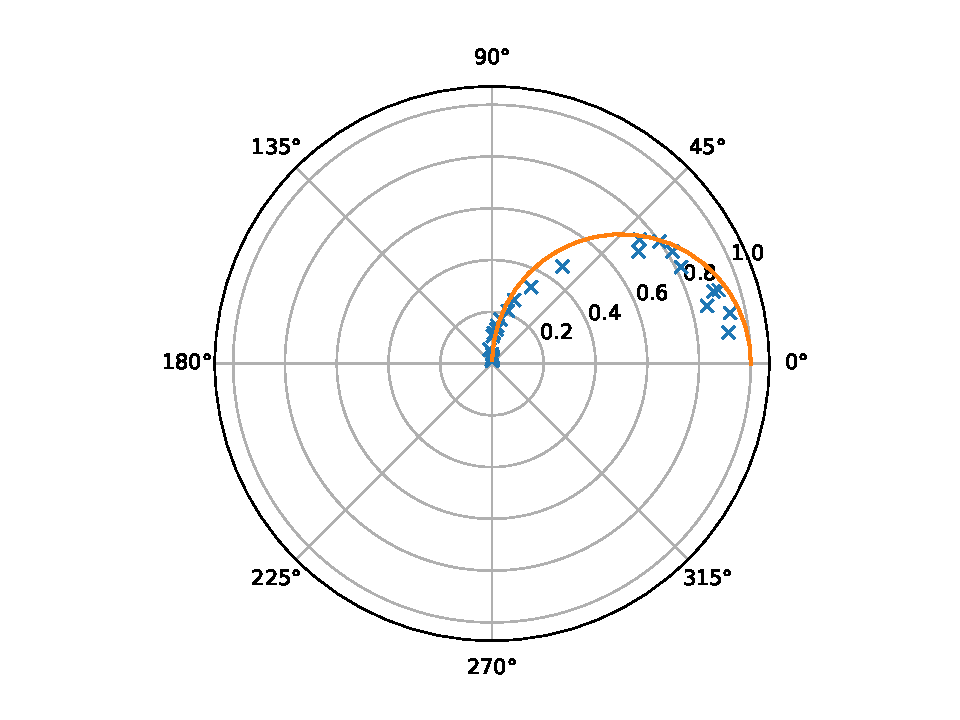
\includegraphics[width=0.8\textwidth]{pl.pdf}
  \caption{Polarplot zur Beobachtung der Phasenverschiebung zwischen der Generator- und Kondensatorspannung.}
  \label{Polarplot zur Beobachtung der Phasenverschiebung zwischen der Generator- und Kondensatorspannung.}
\end{figure}
%\FloatBarrier
%
%
Um die Integrierbarkeit der RC-Spannung zu zeigen wird der Erwartungswert mit dem Realwert vom Oszilloskop verglichen. Da sich Erwartungs- und Realwert decken ist gezeigt das die RC Spannung integrabel ist.
\begin{figure}[h!]
 \centering
 \begin{subfigure}{0.48\textwidth}
  \centering
  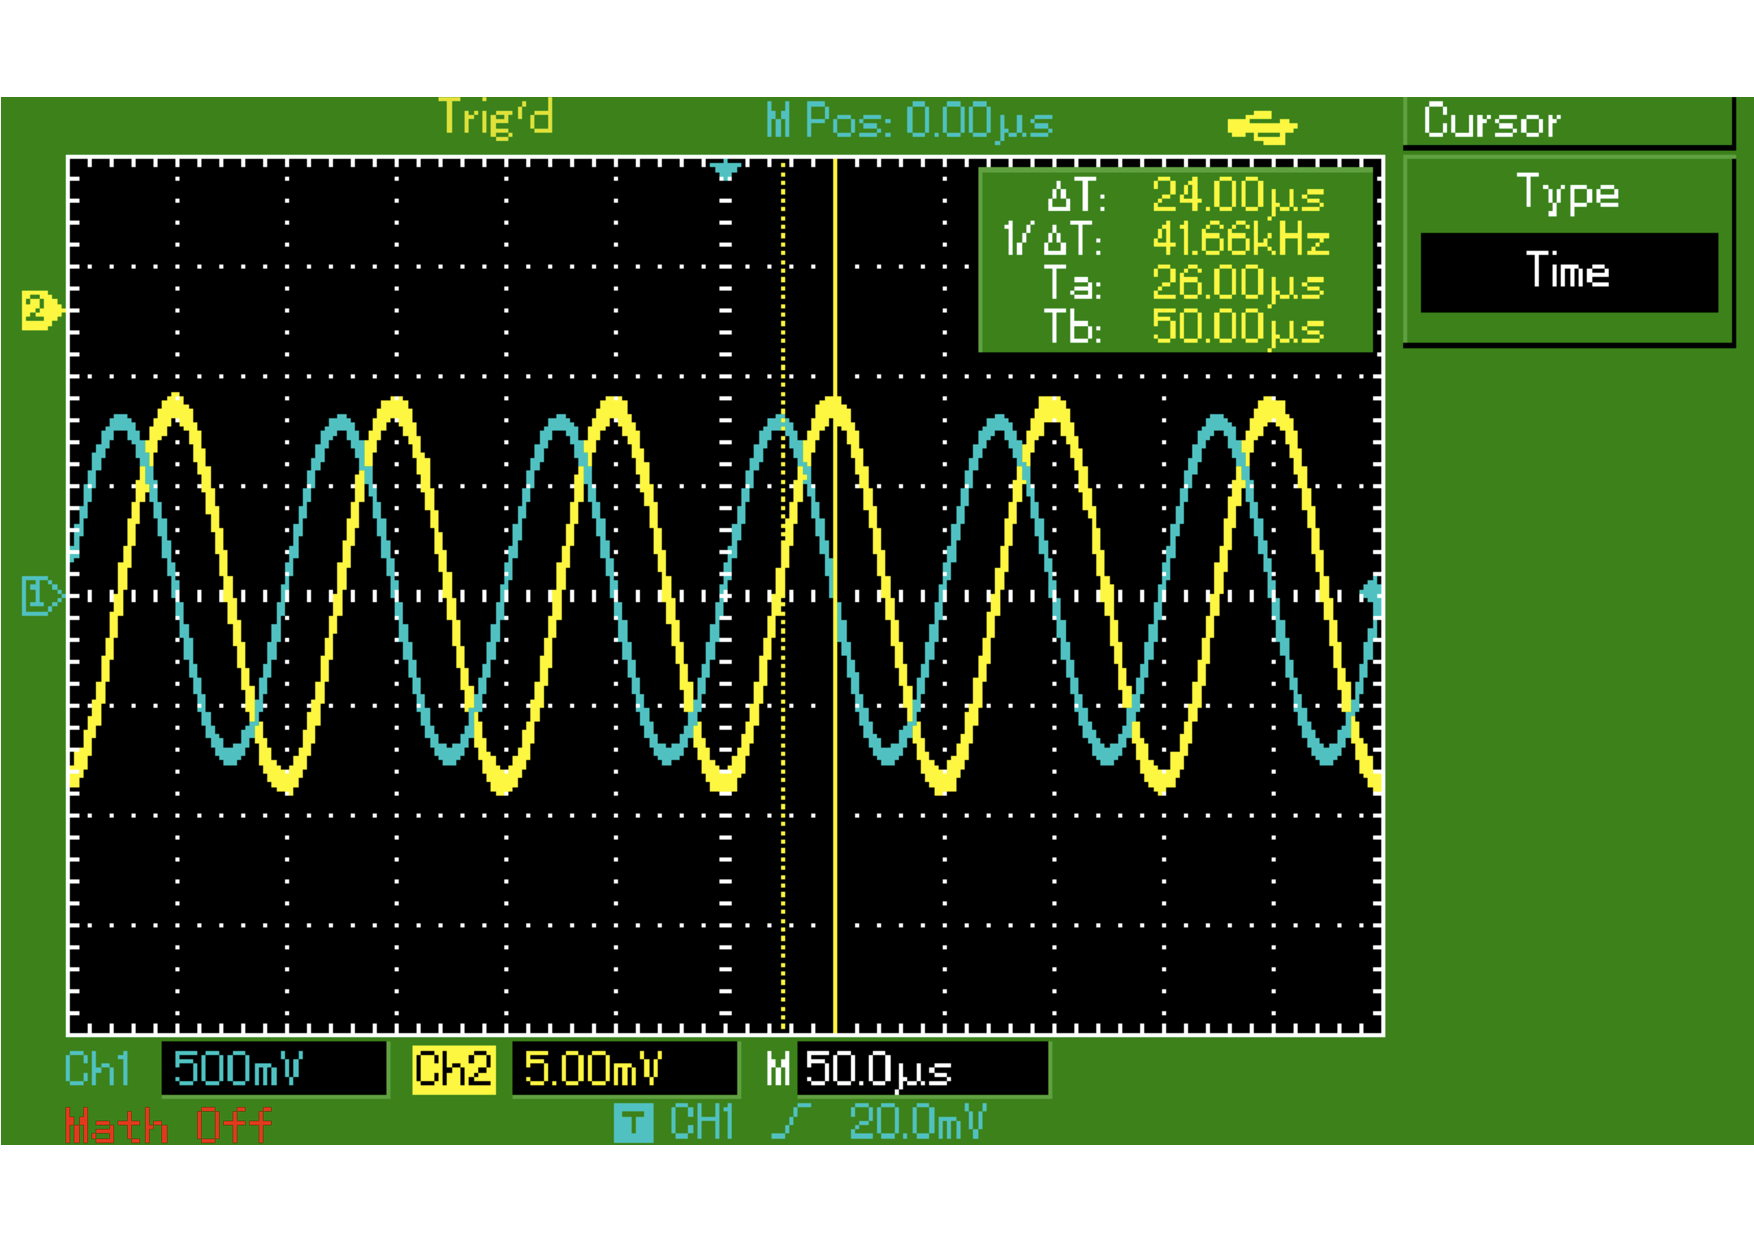
\includegraphics[width=\textwidth]{Oszilloskop1.pdf}
  \caption{Sinusspannung integriert}
  \label{fig:intsin}
 \end{subfigure}
 \begin{subfigure}{0.48\textwidth}
  \centering
  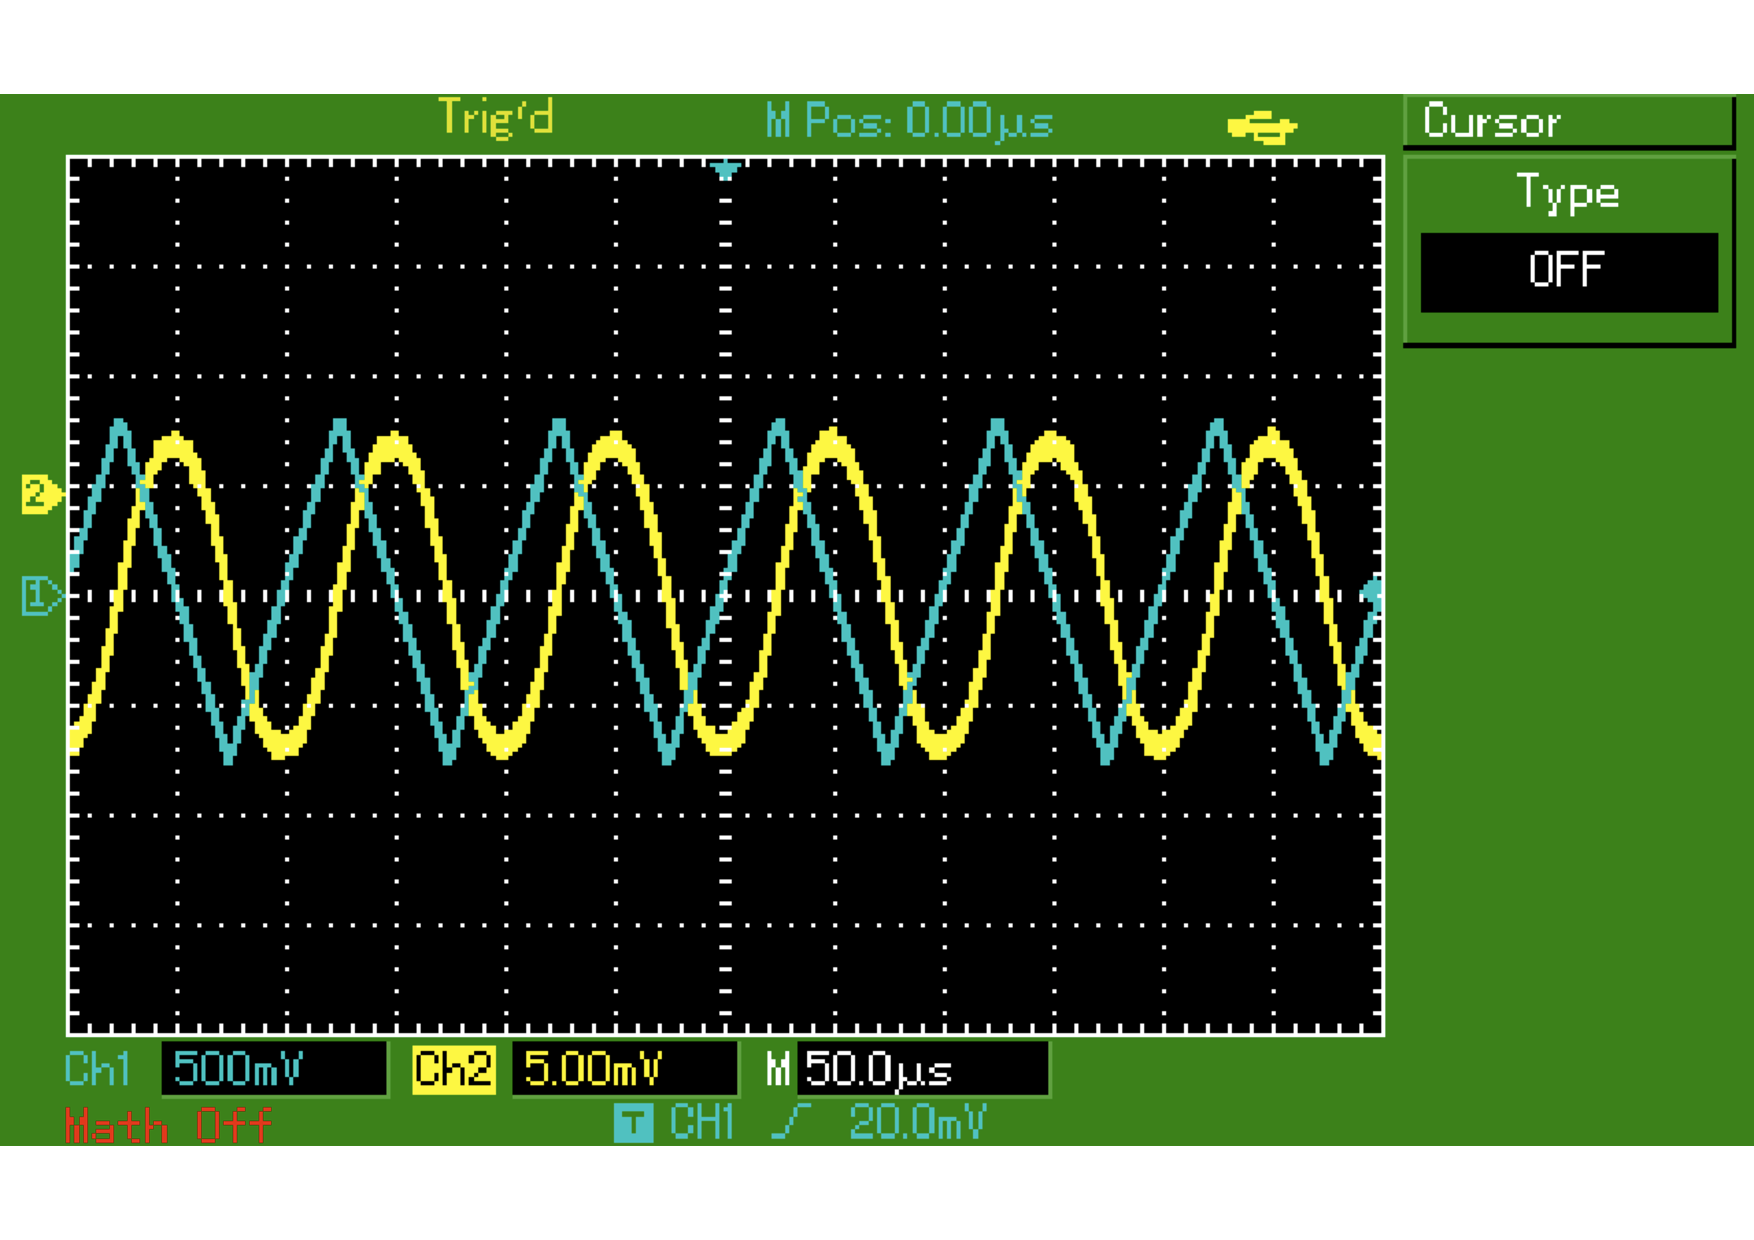
\includegraphics[width=\textwidth]{Oszilloskop2.pdf}
  \caption{Dreiecksspannung integriert}
  \label{fig:90gradnormal}
 \end{subfigure}
% \caption{Spannungsverläufe an dem Mischer}
% \label{fig:000090}
\end{figure}

%\begin{figure}
%  \centering
%  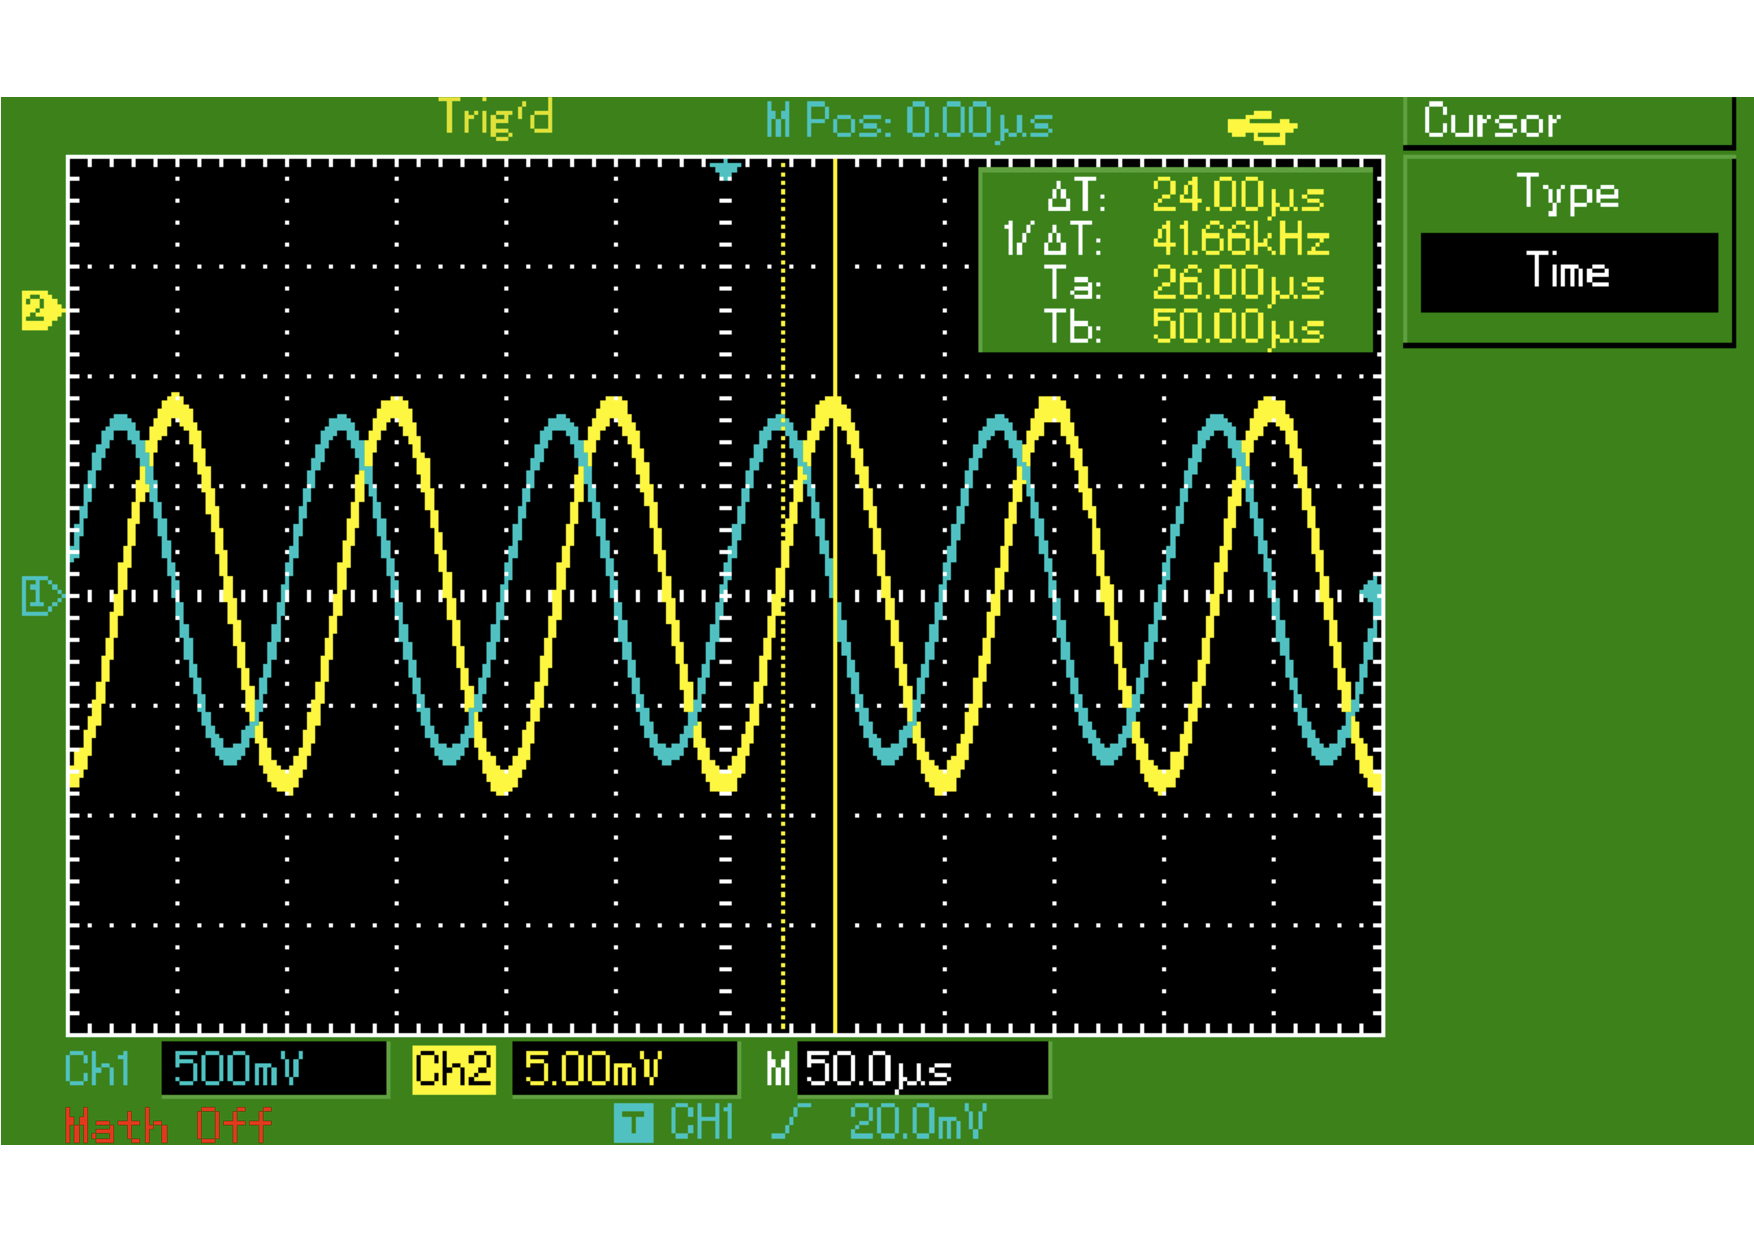
\includegraphics[width=\textwidth]{Oszilloskop1.pdf}
%  \caption{Sinusspannung integriert}
%  \label{fig:intsin}
%\end{figure}
%\begin{figure}
%  \centering
%  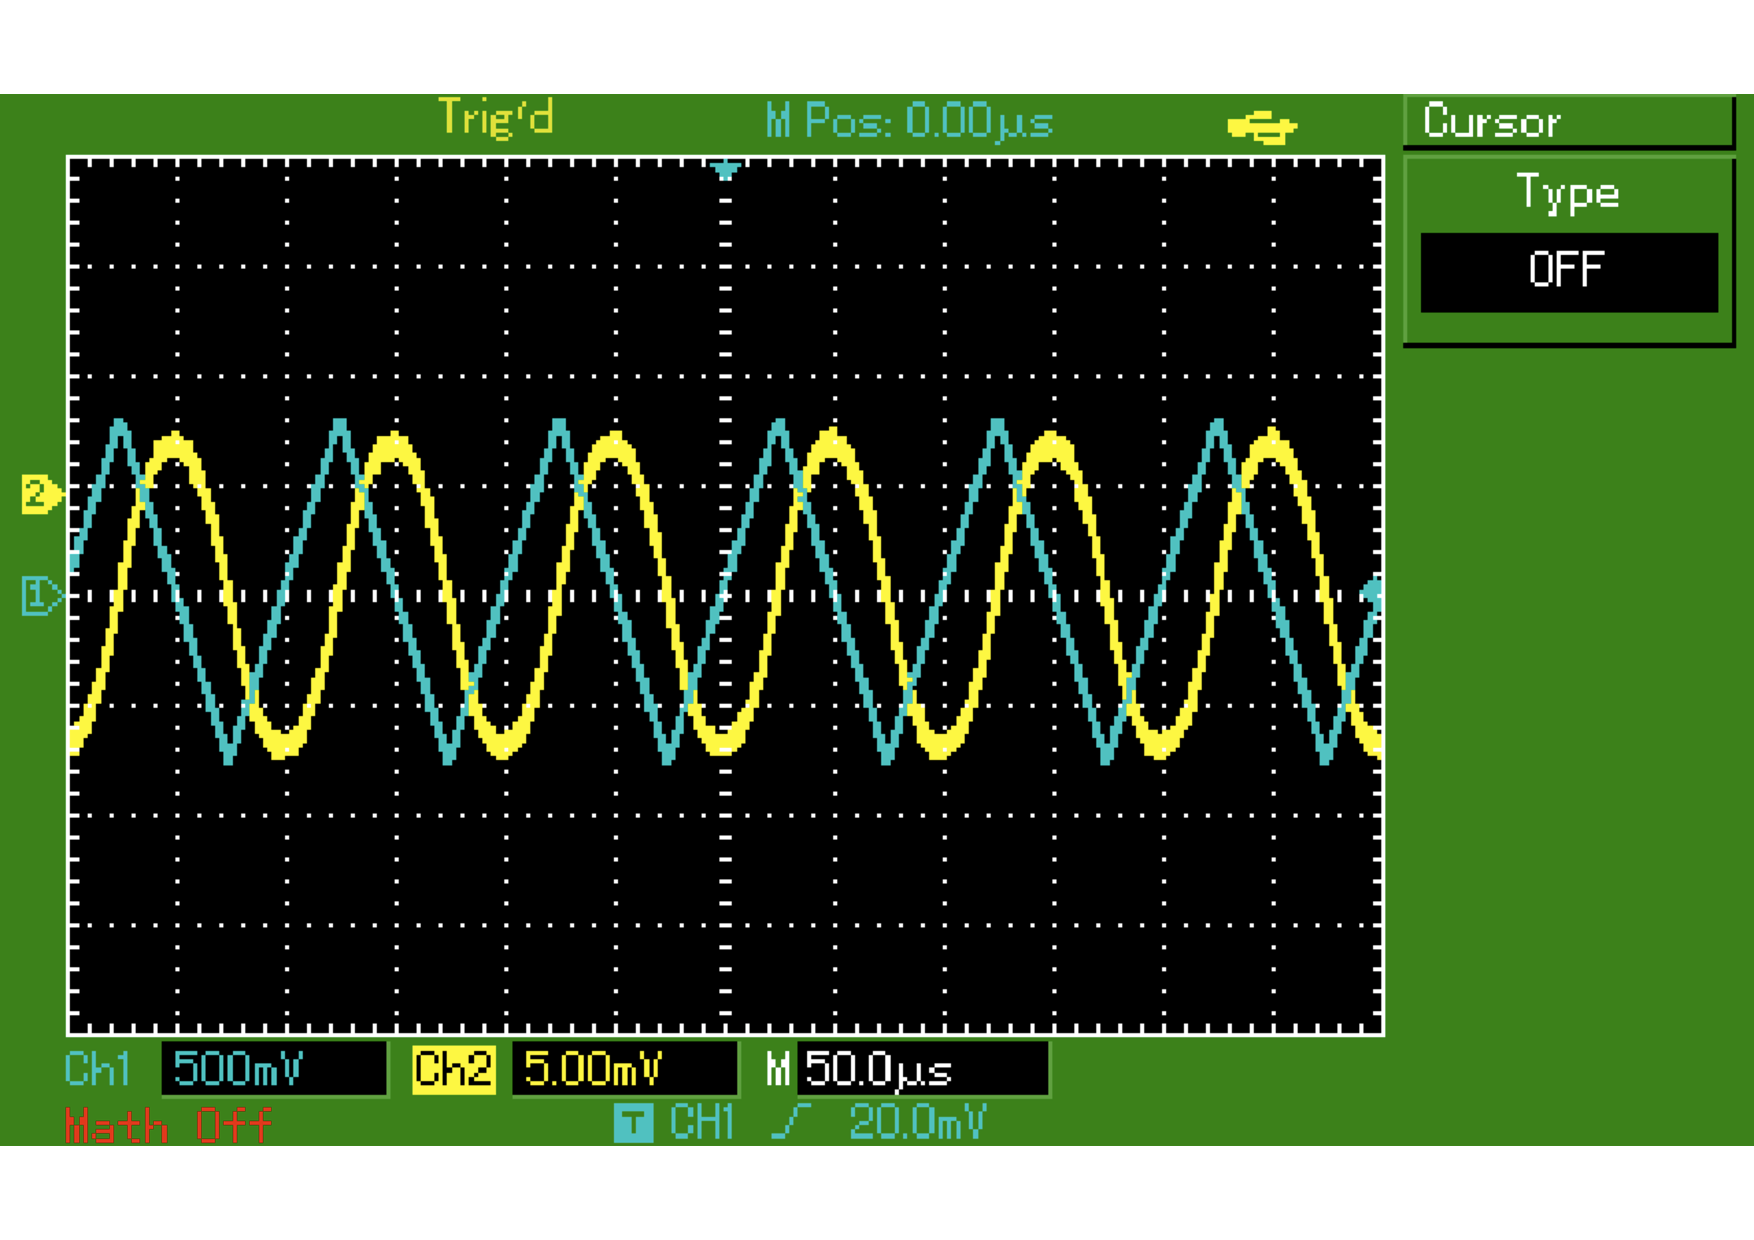
\includegraphics[width=\textwidth]{Oszilloskop2.pdf}
%  \caption{Dreiecksspannung integriert}
%  \label{fig:intdrei}
%\end{figure}
\begin{figure}
  \centering
  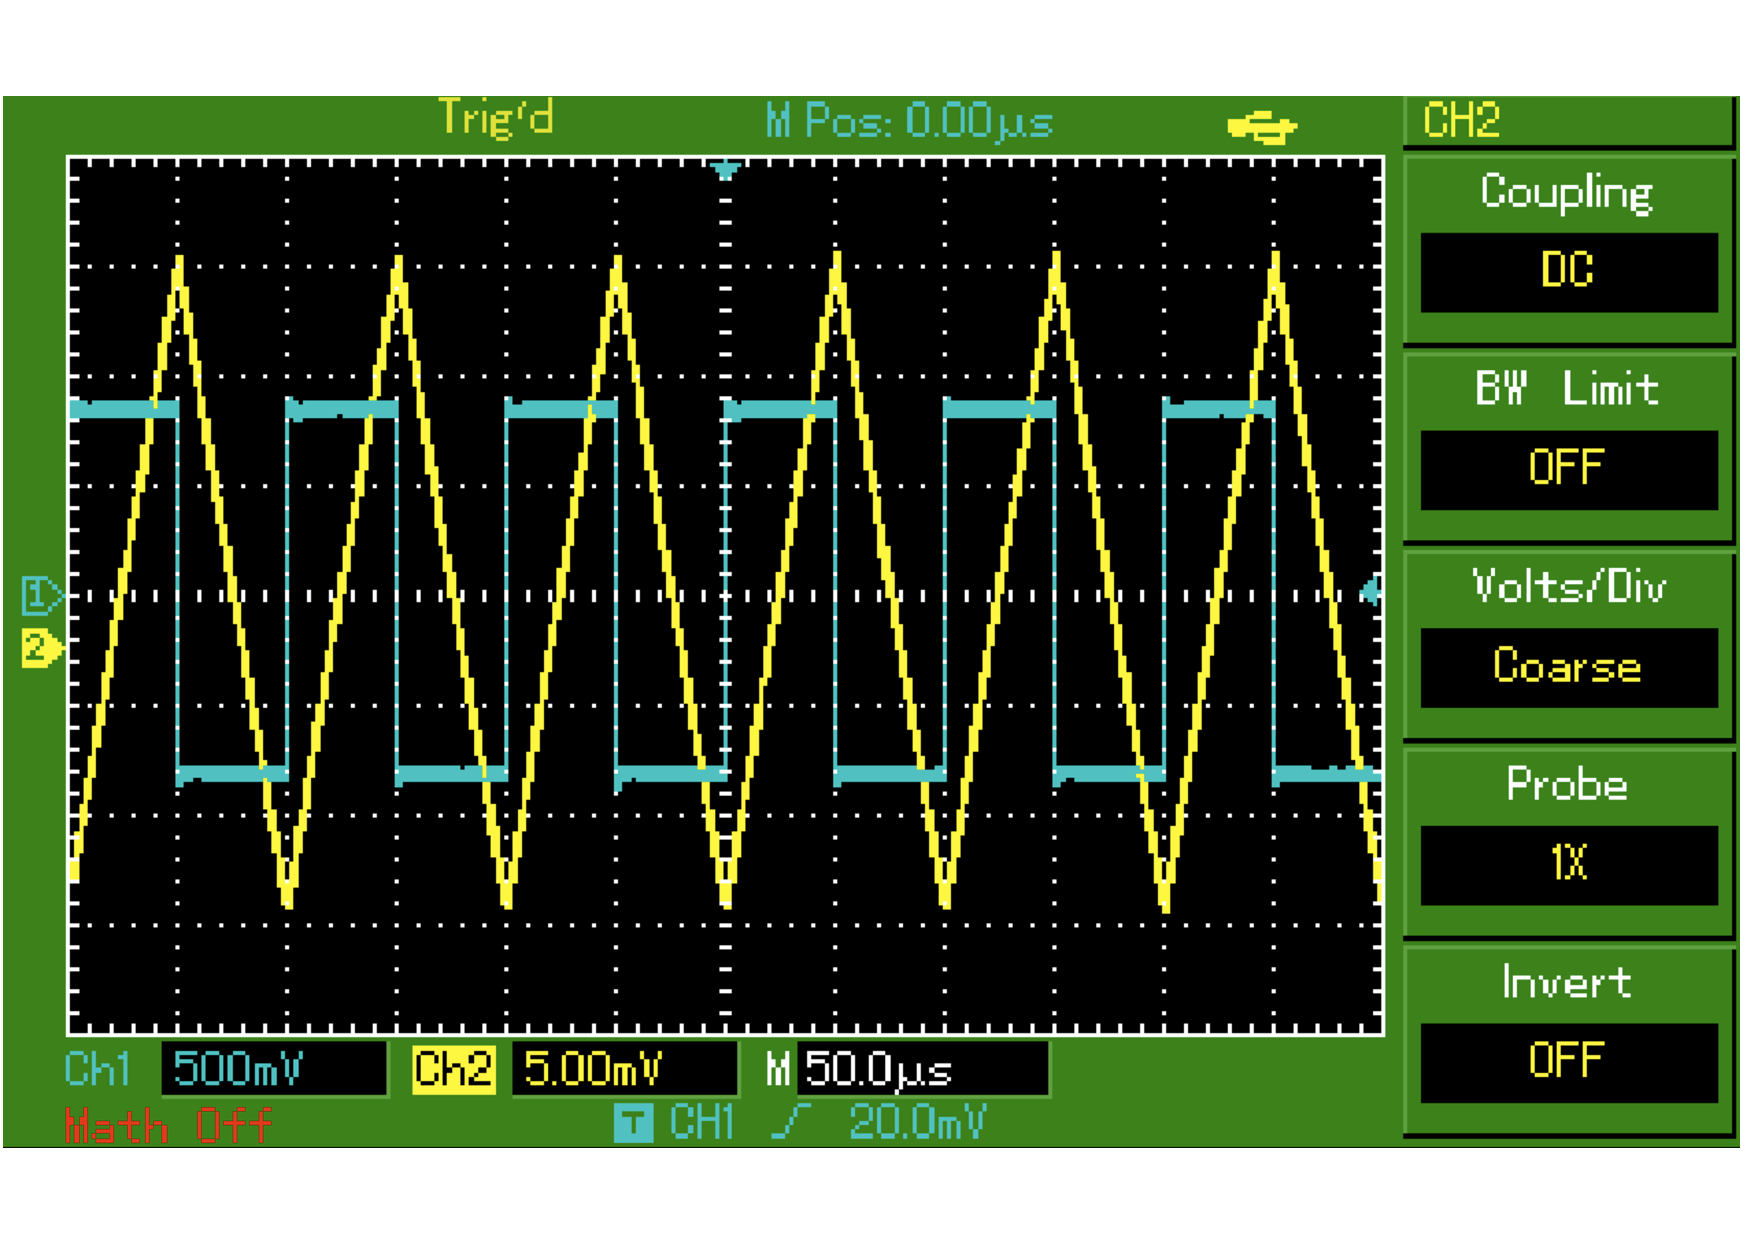
\includegraphics[width=0.48\textwidth]{Oszilloskop3.pdf}
  \caption{Rechteckspannung integriert}
  \label{fig:intrecht}
\end{figure}
\FloatBarrier
%
%
%
